\section{Sorting on a Grid Computing System}
To effectively sort large amounts of data on a distributed system, the following considerations must be made: 
\begin{itemize}
\item How to divide the data into tasks that can be sent to the worker nodes
\item Which algorithms the workers should use to sort those tasks
\item How to merge the sorted packages into one list
\end{itemize}

The above considerations naturally lead to a divide-and-conquer design process. Bucket Sort was used to divide the data and then merge it back together, and Quicksort was chosen as the worker-side sorting algorithm.

\subsection{Distribution of Data to Worker Nodes} \label{sub:modelSplitData}
The master must split the data into tasks for the workers to process. Ideally, these tasks should be of roughly equal size (as discussed in Section \ref{sec:benchmarking}), not so large that they overwhelm the workers, and not so small that the communication overhead becomes larger than the data processing time.

Traditional divide-and-conquer algorithms like Merge Sort and Quicksort divide the data into as many parts as there are elements, and then gradually combine them until there are two parts left to merge. Simply sending these parts to workers will have communication overhead in the beginning, as packets are very few bytes in size, and gradually the problem will shift to workers being overloaded as packets become almost as large as the original data. 

A much better alternative is to divide the data into a series of intervals called "buckets", as shown in Figure \ref{fig:bucketsort}. In the figure, the buckets range between 0 and 49, and there are five buckets. The first bucket should contain all the numbers between 0 and 9, the second bucket should contain all the numbers between 10 and 19, and so on. The correct bucket can be calculated as $\lfloor\frac{\text{Element}}{\text{Bucket interval}}\rfloor$. This process can be done while the file is being loaded, and has a complexity of O($n$) \cite{Introduction_to_algorithms}. This process has the disadvantage of only being effective on uniform distributions. For example, a Gaussian distribution will lead to large buckets in the middle of the data range, and small buckets near the edges, which is contrary to the goal of uniform-sized data packages. A possible mitigation could be dynamically-ranged buckets, where a bucket that would otherwise contain too much data could be split up into more reasonably-sized buckets, but this is not implemented in this project.

\begin{figure}[h]
    \centering
    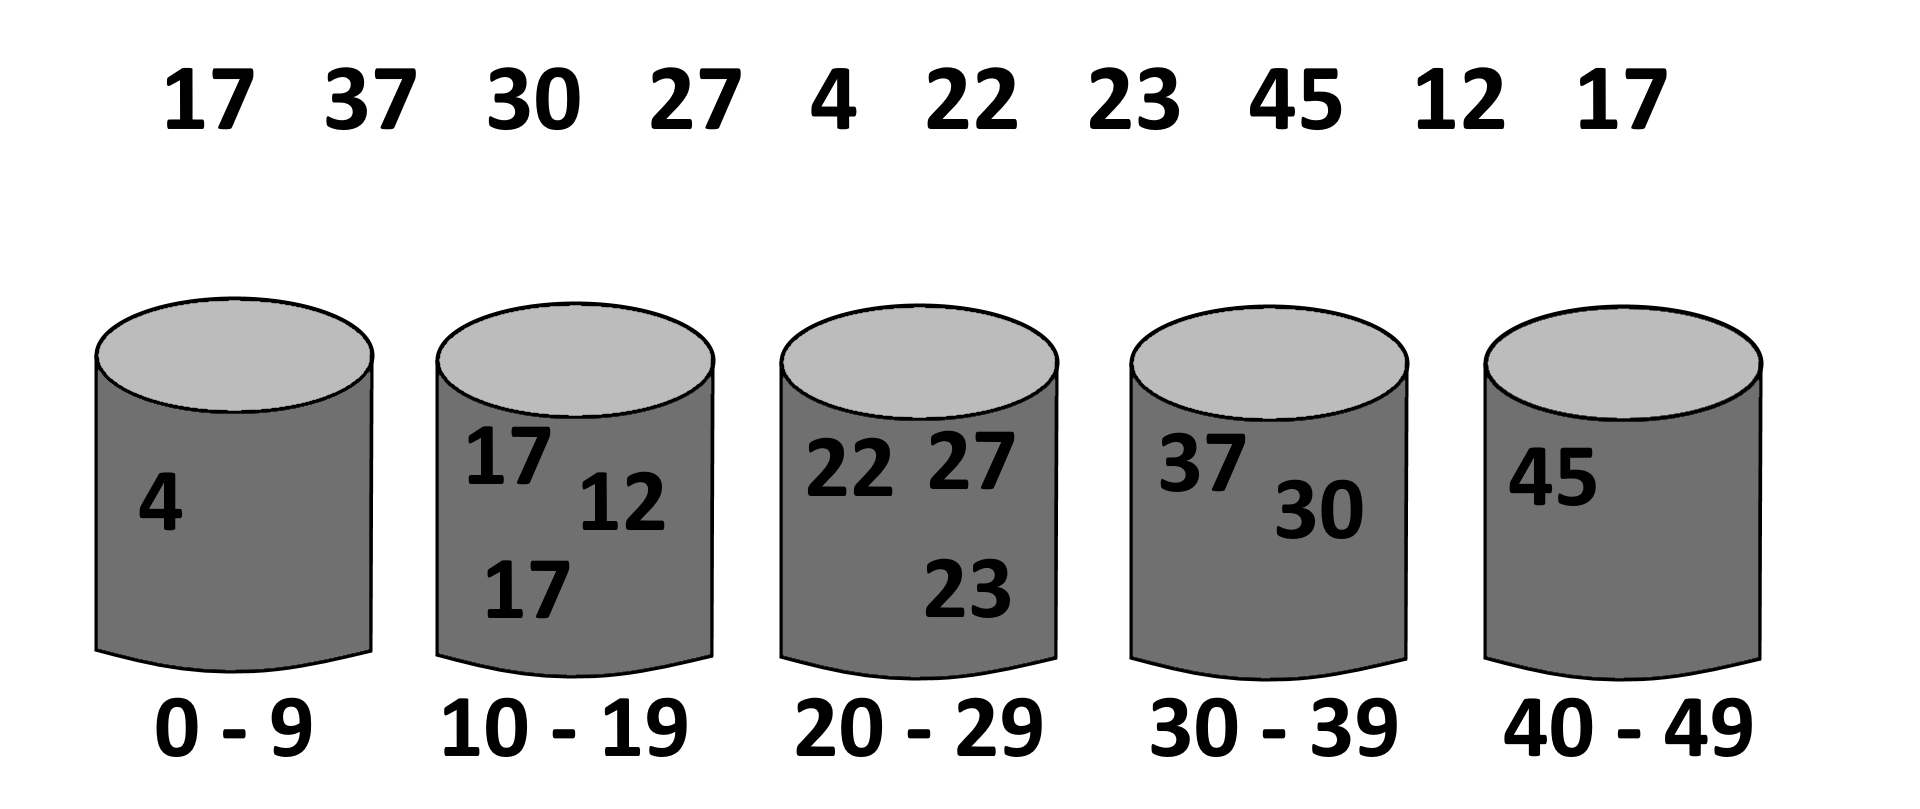
\includegraphics[scale=0.25]{figures/Bucketsort.png}
    \caption{An example of bucket sort working on a list and sorting it into 5 buckets.}
    \label{fig:bucketsort}
\end{figure}


\subsection{Sorting of Local Data by Worker Nodes} \label{sec:quicksortDesc}
Frequently, Quicksort is compared to other sorting algorithms, like Mergesort and Heapsort. This is because they share many similarities and excel in similar tasks. The three algorithms all have an average time complexity of O($n\,log\,n$), making them well-suited for efficiently sorting large data sets \cite{Algorithm_sorts_stanford}. Although all three have an average time complexity of O($n\,log\,n$), their worst case time complexities vary. Quicksort has a worst-case time complexity of O($n^2$) while Mergesort and Heapsort both have one of O($n\,log\,n$). Despite this, Quicksort is still typically considered the fastest, when taking hardware considerations into account \cite{Quicksort_better_answer}.


Another important distinction between the sorting algorithms is their space complexity. Heapsort and Quicksort are both algorithms that can perform sorting in-place, meaning they directly manipulate the data they are working with and hence, do not require any extra memory \cite{In-place_guide}.

\subsubsection{How Quicksort works} \label{HowDoesQuicksortWork}
Quicksort is an algorithm that uses the divide-and-conquer strategy. The algorithm works by choosing a pivot point and then running through all the numbers and dividing them into sub arrays of elements smaller than or bigger than the pivot point. Once this step is completed, the pivot point should be sorted correctly in relation to the smaller or larger numbers. This process is then being repeated until every element is sorted. The performance of the algorithm is significantly influenced by the way the pivot point is chosen. Several commonly preferred options include choosing the first or last element, selecting a random element, or using the median of the first, middle, and last element as the pivot point.


The pseudo-code in algorithm \ref{quicksort_algorithm} shows how the Quicksort algorithm can be implemented:

\begin{algorithm} [H] 
\caption{quicksort(left = $0$, right = Data.length $- 1$)} \label{quicksort_algorithm}
\SetAlgoNoLine

\uIf{left $<$ right}{
pivotIndex = genRandomInt(left, right) 

pivot = data[pivotindex] 

partitionIndex = HOARE-PARTITION(pivot,left,right)

quicksort(left, partitionIndex)

quicksort(partitionIndex $+ 1$, right)

}
\Else{
\textbf{return}
}

\end{algorithm}

At the beginning of the sorting process the variables "left" and "right" are initialized with placeholders, where "left" is set to 0 and "right" is set to the length of the data minus one. If "left" is smaller than "right", a pivot point is randomly selected between "left" and "right". Afterwards, the variable "pivot" is set to the value of "data[pivot]" 

Next, the code HOARE-PARTITION (as described in Algorithm \ref{Partition}) runs and returns the index of the partition point to the variable "partitionIndex". This then splits the data in two subarrays, one with every number under the pivot index, and another with every number over the pivot index. The Quicksort algorithm then calls itself twice, once for each of the subarrays created.
\\
Pseudo-code \ref{Partition} shows how Hoare's partition can be implemented \cite{Introduction_to_algorithms}:

\begin{algorithm} [H] \caption{HOARE-PARTITION(pivot, left, right)}\label{Partition}
\DontPrintSemicolon
\SetAlgoNoLine
    x $=$ pivot\\
    i $=$ left $- 1$\\
    j $=$ right $+ 1$\\
     \While{TRUE}{
     \RepeatUntil{A[j] $\le$ x}{j$=$j$-1$}
     \RepeatUntil{A[i] $\ge$ x}{i$=$i$+1$} 
     \If{i $<$ j}{
       Exchange A[i] with A[j]
    }
     \Else{
        \textbf{return J}
    }
}

\end{algorithm}

The pseudo-code demonstrates a single call of the partition function on an unsorted list, using the two pointer approach, also known as Hoare's partition scheme. The way it works is by having two pointers, one at the end and one at the beginning of the array. The pointer at the end goes through all the elements on the right side of the pivot point until it finds a number that is smaller than the pivot. The pointer at the beginning of the array does the same thing afterwards, from the left side of the pivot point, until it finds a number bigger than the pivot. When both conditions are met, the algorithms swaps the two numbers and then continues to check every number until they meet each other. When the algorithm terminates it returns the partition index \cite{hoare-partition}.

\subsection{Merge of Sorted Data at the Master Node}
Once all the workers have finished their tasks and sent the finished buckets back, the buckets must be merged. Because they were split into buckets, where the elements of bucket $n$ are always greater than those of bucket $n-1$, the merge procedure is as simple as concatenating the buckets. 